% !TEX encoding = UTF-8
% !TEX program = pdflatex
% !TEX root = InformationRetrieval.tex
% !TEX spellcheck = it-IT

\section{Search Engine Optimization}

Il linguaggio HTML non è stato pensato per i motori di ricerca e per farci reperimento dell'informazione. Tutto è iniziato per trovare un modo di rappresentare dei documenti che funzionasse anche per non informatici.

\subsection{Ranking delle pagine}

Il \textbf{ranking statico} viene definito nel momento dell'indicizzazione effettuando l'analisi del contenuto e dei link presenti nella pagina web.

L'indicizzazione e l'uso dei link, se fatta in modo accorto, la struttura della pagina deve riflettere la qualità, l'autorevolezza e la popolarità di una pagina web. 
Migliore è la qualità della pagina, maggiore è il rank statico calcolato dal motore per la pagina.

Da notare che se un motore di ricerca fornisce tra i primi risultati una pagina autorevole non implica che è un motore che funziona bene.

Il \textbf{ranking dinamico} viene calcolato combinando la query con il ranking statico delle pagine. Vengono quindi prese in considerazione alcuni fattori che dipendono dalla query come la presenza dei termini e le loro prossimità.
Le modalità di ranking statico e dinamico variano da motore a motore.

Tuttavia, anche se ci sono vari algoritmi, ci sono due comportamenti tipici:

\begin{itemize}
	\item \textbf{Testo delle ancore}: l’efficacia del reperimento può essere aumentato sfruttando il testo delle ancore
	\item \textbf{Novità} o \textbf{Novelty}: piuttosto che restituire tante pagine di uno stesso sito, viene fornita solo quella principale. In modo da fornire dei risultati che sono il più vari possibili.
\end{itemize}

\subsection{SEO}

L'idea è quella di aumentare il ranking delle pagine in modo che il proprio sito finisca tra i primi risultati del motore di ricerca.
Infatti, un buon posizionamento permette una maggiore visibilità e sperabilmente aumenta il traffico in entrata del sito.
Ovviamente un prerequisito fondamentale è quello che la pagina web sia indicizzata dai principali motori di ricerca.

Tipicamente gli aspetti SEO sono strettamente legati alla qualità del sito web. Maggiore è la qualità, maggiore è la probabilità che il sito sia ben posizionato in una ranking list.

La qualità del sito dipende:

\begin{itemize}
	\item dai contenuti che devono essere buoni e scritti correttamente.
	\item dalla frequenza di aggiornamento del sito, che deve essere specificata sia nei meta-tag, che sotto forma di data presente negli articoli.
	\item dalla manutenzione della pagina. \`E strettamente legato all'aggiornamento.
	\item dal codice, che deve essere pulito e ben formato. Non devono essere presenti parti di codice ridondanti e il codice deve essere scritta con una sintassi corretta.
	\item dall'autorevolezza della pagina, la quale dipende dai link che ci sono in entrata verso il sito.
\end{itemize}

Ovviamente essere visti da un motore di ricerca permette di essere visti da molte persone e quindi produce valore per le attività commerciali.

Da notare che \textbf{nessuna} pratica di SEO ha un'efficacia garantita.
Questo perché tutte le tecniche di SEO sfruttano un approccio empirico che interpreta in modo approssimato il comportamento dei motori di ricerca e cerca di mettere in atto delle azioni che possano essere utilizzate opportunamente da questi.

Quindi noi possiamo solamente cercare di migliorare il sito e i suoi contenuti, nella speranza che i motori di ricerca ci ritengano autorevoli, senza nessuna certezza, questo perché i motori di ricerca utilizzano molti criteri per stabilire il rank di una pagina.

Alcune caratteristiche che vengono giudicate positivamente dai motori di ricerca sono:

\begin{itemize}
	\item Presenza di uno o più termini della query nel tag \texttt{<title>} della pagina.
	\item Presenza di un termine della query nel \texttt{<body>}.
	\item Utilizzo del tag \texttt{<strong>} attorno ad un termine della query.
	\item Presenza di un termine di ricerca in un elemento \texttt{<heading>} o \texttt{<a>}. Un ancora in uscita con un termine della query viene ben vista, perché il ragionamento è quello del ``\textit{l'autore non manderebbe mai via l'utente dal suo sito se l'informazione non è molto importante, quindi il contenuto della pagina che contiene l'ancora deve essere ben fatto}''.
	\item Autorevolezza dei link che puntano verso la nostra pagina. Può essere determinata utilizzando delle liste di domini ritenuti autorevoli.
	\item Velocità di caricamento del tipo. Ad esempio, le immagini devono essere delle dimensione corrette, in modo che il loro caricamento sia veloce. Lo stesso vale per tutti gli altri file multimediali.
\end{itemize}

Queste caratteristiche sono state derivate dallo studio della letteratura, anche se limitata, e da prove pratiche.

Altri aspetti che invece si è visto che vengono considerati negativamente sono:

\begin{itemize}
	\item La presenza dei trattini (hypens) nell'URL. Non si sa bene il perché.
	\item Lunghezza dell'URL. Se l'URL è lungo, vuol dire che si sta andando in profondità del sito e quindi il contenuto è stato messo in disparte, appunto perché è in profondità.
	\item Lunghezza del tag \texttt{<title>}, non deve essere né troppo lungo, né troppo corto.
	\item Quantità di pubblicità presente nella pagina. Se ce n'è troppa la pagina, questa viene penalizzata.
	\item Numero di immagini e video. Non solo la pesantezza, ma anche la dimensione.
\end{itemize}

Ci sono poi altri aspetti che influenzano il ranking. Questi si dividono in due categorie:

\begin{itemize}
	\item \textbf{On the page}: sono quelli sotto il controllo dell'autore della pagina, come il contenuto, la struttura HTML e l'architettura del sito.
	\item \textbf{Off the page}: sono fattori esterni non direttamente controllabili, come la qualità dei link che puntano al nostro sito, l'autorevolezza dei contenuti e la reputazione social.
\end{itemize}

\subsubsection{On the page}

Uno dei fattori più importanti è il contenuto della pagina, il quale deve essere originale. 
I contenuti copiati, in parte o del tutto, influiscono negativamente sul ranking e contribuiscono a far diminuire l'autorevolezza e la credibilità di un sito. Il contenuto dovrebbe essere \textbf{unico}, \textbf{diverso} e \textbf{utile}.

\begin{figure}[htbp]
	\centering
	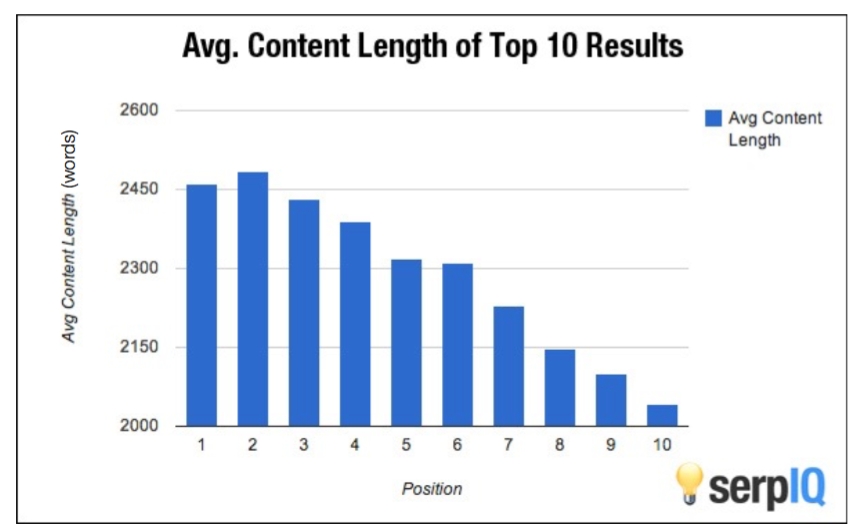
\includegraphics[width = 0.5\textwidth]{images/l23-fig-1}
	\caption{Contenuti lunghi e approfonditi sono in genere preferiti}
\end{figure}

Alcuni motori di ricerca calcolano il livello di leggibilità dei siti web, dove un alto livello di leggibilità (basso valore per il motore) indica un sito con contenuti ``\textit{facili e adatti alle masse}'' mentre un basso livello di leggibilità indica ``\textit{contenuti più complessi e elitari}''.
Non è chiaro cosa sia preferibile, ma il ranking può essere categorizzato in base a questo indice.

Anche la presenza \textbf{parole chiave} relative all'argomento del sito all'interno del contenuto è importante.

\paragraph{Title} Il tag \texttt{<title>} gioca un ruolo molto importante, sia a livello di ranking, sia perché viene mostrato tra i risultati della ricerca che vengono forniti all'utente.
\`E quindi buona norma utilizzare dei titoli correlati all'argomento della pagina, che contengano delle parole chiavi e non troppo lunghi. All'interno del titolo può anche comparire il brand del sito.

\paragraph{Meta-tag}Anche i meta-tag della sezione \texttt{head} sono molto utilizzati dai motori di ricerca e vengono utilizzati per popolare gli snippet presenti nella pagina dei risultati.
Non c'è la certezza, ma sembra che vengano apprezzati dai motori di ricerca.

\paragraph{Dimensione e immagini} La dimensione in byte della pagina gioca un ruolo fondamentale, perché viene presa sia in considerazione dai motori di ricerca che dagli utenti del sito, è quindi importante che ci sia un equilibrio tra testo e immagini.
La presenza delle immagini deve essere anche limitata perché i crawler raccolgono solo una parte della pagina, e se la parte della pagina comprende tante immagini, queste non forniscono informazioni utili.
\`E inoltre sconsigliato utilizzare delle immagini come testi per i link.

\paragraph{Struttura della pagina} I crawler preferiscono le pagine poco profonde, con una struttura semplice perché risultano più semplici da indicizzare. \`E quindi sconsigliato utilizza le tabelle HTML ed è incentivato l'uso dei \texttt{<div>} opportunamente stilati con i CSS.
Tutto lo stile della pagina dovrebbe essere contenuto in un file CSS seprato, sia per una questione di separazione della presentazione dal contenuto, sia perché questo alleggerisce le dimensioni della pagina.
\`E inoltre importante prestare attenzione alla \textbf{site crawlability} della pagina, ovvero i contenuti dovrebbero essere facilmente accessibili dal crawler, quindi attenzione al JavaScript che potrebbe nascondere delle informazioni e niente Adobe Flash.
Sempre per facilitare il lavoro del crawler è utile specificare nel file \texttt{robot.txt} quali pagine non indicizzare, questo perché il tempo del crawler sul sito è limitato ed è meglio che eviti di sprecarlo su pagine inutili. L'utilizzo di una sitemap può agevolare ulteriormente il crawler.

\paragraph{Contesto} Il contesto geografico, temporale, sociale in cui viene effettuata una ricerca viene preso in considerazione dai motori di ricerca. Quindi possono influire positivamente sul ranking i seguenti fattori:

\begin{itemize}
	\item Indicare la città o lo stato nel tag \texttt{<title>}
	\item Il fatto che la regione del dominio o l'indirizzo fisico del server coincida con la regione in cui è stata effettuata la ricerca.
	\item Presenza della città o stato nei tag di heading.
\end{itemize}

\subsubsection{Off the page}

Anche i social network influiscono sul ranking di una pagina, infatti se una pagina viene spesso condivisa, twittata, riceve like ed è attiva sui social, il suo ranking aumenta.

L'altro fattore off the page che influisce principalmente sul ranking è l'autorevolezza del sito, determinata dai contenuti, dalla reputazione dell'autore e dallo storico del dominio. Domini più vecchi sono preferiti in quanto sono resistiti nel tempo.


\subsubsection{Riferimenti utili}

\begin{itemize}
	\item \url{http://searchengineland.com/}
	\item \url{http://moz.com/search-ranking-factors/}
\end{itemize}








